\documentclass[10pt, oneside]{article}   	% use "amsart" instead of "article" for AMSLaTeX format
\usepackage[a4paper]{geometry}             % See geometry.pdf to learn the layout options. There are lots.
\geometry{letterpaper}                   		% ... or a4paper or a5paper or ... 
%\geometry{landscape}                		% Activate for rotated page geometry

%PACKAGES:------------------------------------------------------------
%\usepackage[parfill]{parskip}    		% Activate to begin paragraphs with an empty line rather than an indent
\usepackage{graphicx}				% Use pdf, png, jpg, or eps§ with pdflatex; use eps in DVI mode
\usepackage[font=small,labelfont=bf]{caption}								% TeX will automatically convert eps --> pdf in pdflatex	

\usepackage{amssymb}
\usepackage{fullpage}
\usepackage{amsmath}
\usepackage{listings}
\usepackage{hyperref}
\usepackage[table]{xcolor}
\usepackage[article]{ragged2e}
\usepackage[T1]{fontenc}
\usepackage[utf8]{inputenc}
\usepackage{geometry}
\usepackage{tikzpagenodes}
\geometry{textwidth=7cm}


\usepackage[T1]{fontenc}

\pdfpagewidth 8.5in
\pdfpageheight 11in
\headheight 0pt
\headsep 0pt
\footskip .25in
\marginparwidth 0pt
\marginparsep 0pt
\oddsidemargin \dimexpr 1in -1.0in
\topmargin \dimexpr 1in -1in			%Top margin global
\textwidth \dimexpr \pdfpagewidth -2\oddsidemargin -2in
\textheight \dimexpr \pdfpageheight -2\topmargin -2in

%SetFonts

%SetFonts

\renewenvironment{abstract}		%Formats the Abstract
 {\normalsize		%abstract text size \normalsize or \small
  \begin{center}
  \bfseries \abstractname\vspace{-.5em}\vspace{0pt}
  \end{center}
  \list{}{
    \setlength{\leftmargin}{1.4cm}%		%sets the margin size
    \setlength{\rightmargin}{\leftmargin}%
  }%
  \item\relax}
 {\endlist}







\begin{document}


\begin{center}
% Title of Lab
\LARGE{\textbf{Assignment One Report}}	%TITLE
\end{center}
\vspace{-1mm}
\begin{flushright}
% Course Code
\large{COSC-363}
\end{flushright}
\vspace{-11mm}
% Name
\large{Benjamin Thurber}			%AUTHOR NAME
\vspace{0mm}
\begin{center}
% Date
\centerline{\large{20, April, 2020}}
\end{center}

\vspace{-10mm}
\begin{flushleft}
ID: 56259636

\end{flushleft}

\begin{center}
\vspace{2mm}
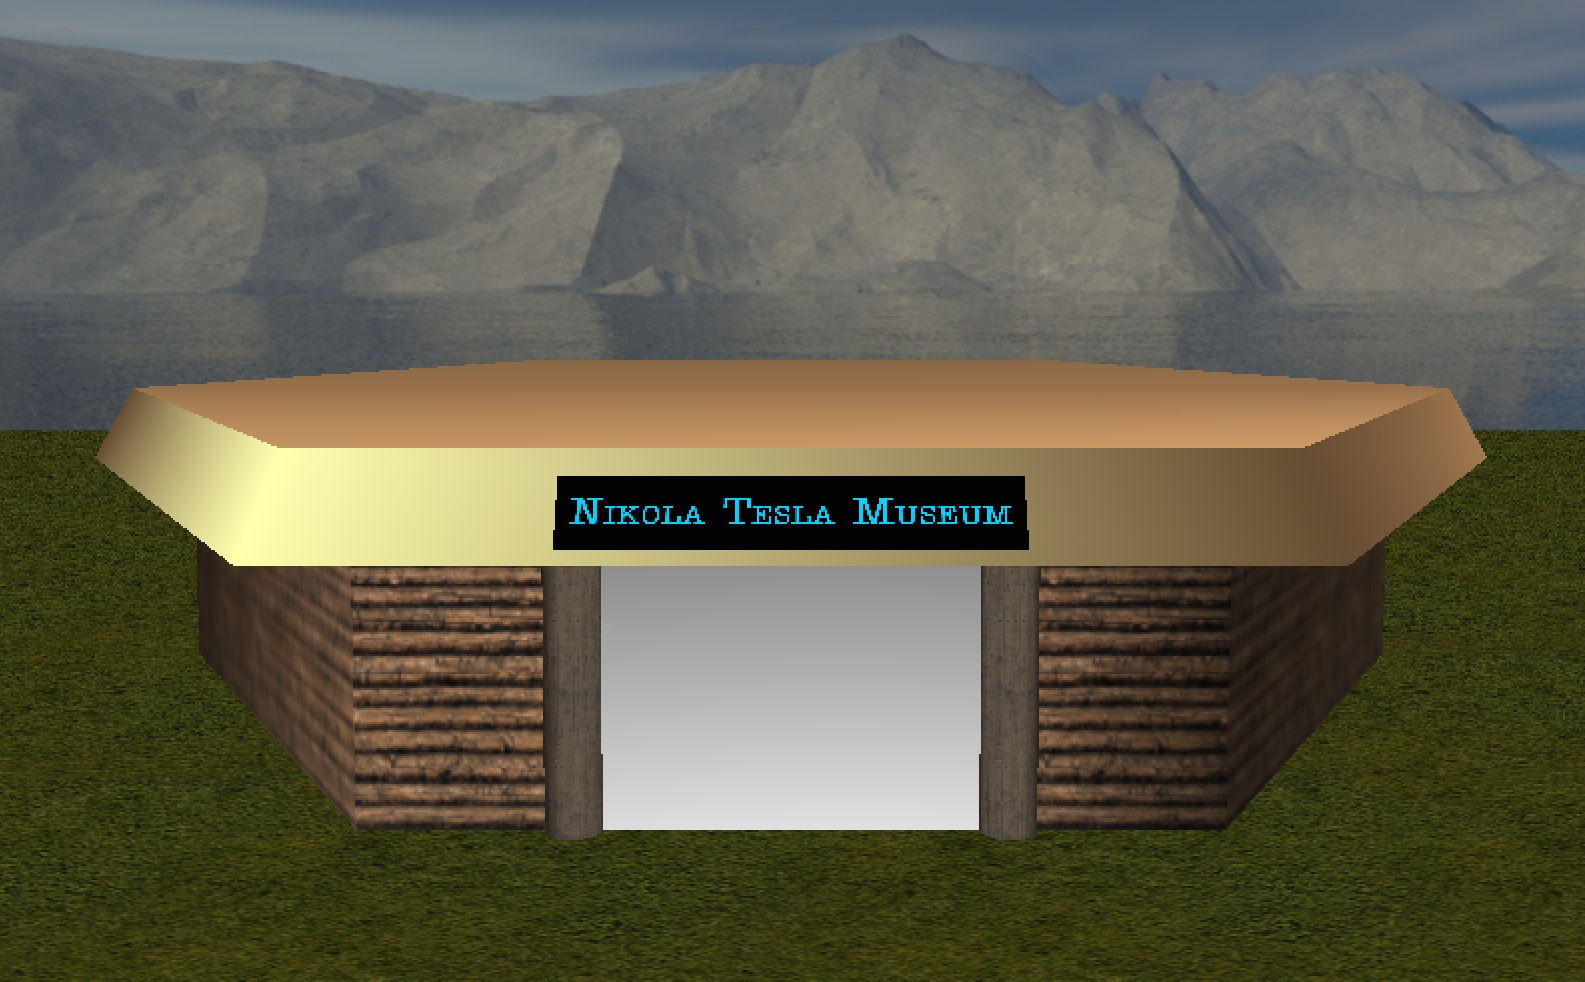
\includegraphics[height=6cm]{building.jpg}   % Image
\end{center}


\vspace{-3mm}
\normalsize

\section{Background}
For my assignment I designed a model of a hexagonal one room museum building that the viewer can walk into and view the exhibits.  The theme of the museum is based around the inventions of the 19-Century scientist Nikola Tesla.  In clockwise order, the first exhibit is a model of the first radio controlled boat.  In the back right corner is a Tesla Coil, a device to produce high voltage electricity.  To the right of the doorway is an electromechanical oscillator attached to a steel beam, supported at both ends.  The oscillator attached to the bar moves up and down, demonstrating the resonant frequency of the beam.

%Three of his inventions (clockwise) are displayed; the first radio controlled boat, the tesla coil and an electro-mechanical oscillator.

\section{Compilation}
The program is configured with a CMakeLists.txt file and cmake.  The program is compiled using make.

\subsection{Requirements}
\begin{itemize}
\item C++
\item freeGLUT / GLUT
\item X11
\item cmake
\item make
\end{itemize}

\subsection{Compile}
cd into Assignment1/ directory and run
\newline \newline
{\small \fontfamily{qcr}\selectfont
cmake ./
\newline
make
}
\newline \newline
which will create a binary file called ``assignment1''.

\subsection{Run}
Run by executing
\newline \newline
{\small \fontfamily{qcr}\selectfont
./assignment1
}



\section{Movement System}
The camera is moved through the scene using the keyboard.  Two key mappings are available which can be \textcolor{red}{toggled between by pressing \textbf{shift-t}.}  $\uparrow$, $\downarrow$, $\leftarrow$, $\rightarrow$ are the arrow keys.
\newline
\subsection{Default strict mappings}
The following is the default and follows the required key mapping in the assignment.
\begin{itemize}
\item $\uparrow$, $\downarrow$ Move forward, backward
\item $\leftarrow$, $\rightarrow$ Look left, right
\item `w', `s' Move right, left
\item `a', `d' Look up, down
\item SPACE BAR Move up
\item `c' Move down
\end{itemize}

\subsection{Custom mappings}
Key mapping that do not follow the assignment guidelines but may be easier to use.
\begin{itemize}   % Change these
\item $\uparrow$, $\downarrow$, $\leftarrow$, $\rightarrow$ Look up, down, left, right
\item `w', `s', `a', `d' Move forward, back, left right
\item SPACE BAR Move up
\item `c' Move down
\end{itemize}

% Image
\begin{tikzpicture}[remember picture,overlay,shift={(current page.north east)}]
\node[anchor=north east,xshift=-0.5cm,yshift=-13cm]{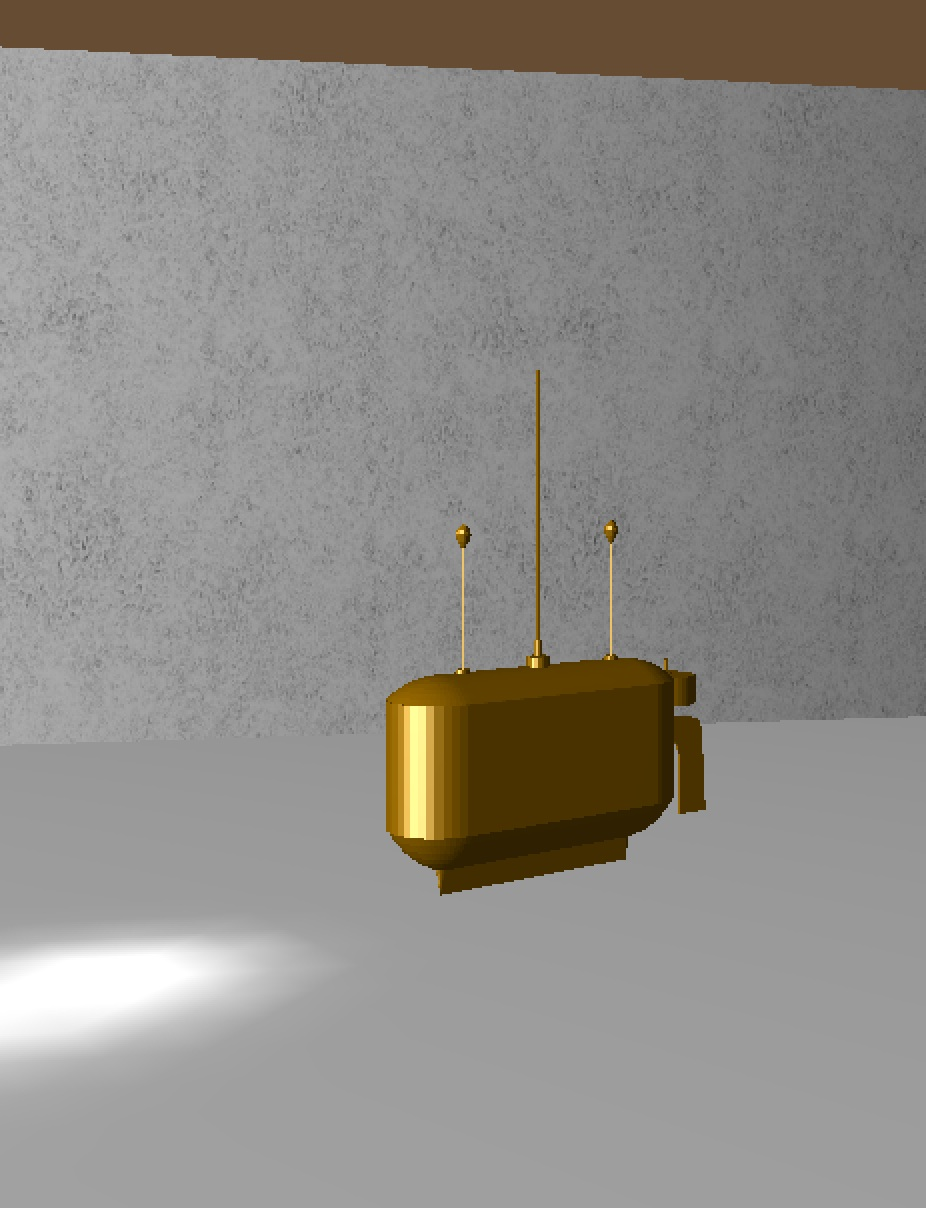
\includegraphics[width=4.5cm]{boat.jpg}};
\end{tikzpicture}

\section{Exhibit Descriptions and Extra Features}
The museum implements the features: Spot light, particle system, surface and animations generated from a formula and skybox, as well as mipmaps.
\subsection{Remote controlled boat}
The model in the left side of the museum is an OFF model that is animated to move in a figure of eight pattern and bob slightly up and down as if it were afloat.  A spot light on the boat illuminates the floor.
\newline
\newline
\textbf{Feature: Mathematical Formula}\hspace{3mm} The boat moves in a figure of eight according to the equation\textsuperscript{[1]} 
\begin{equation}
x^4 = a^2(x^2-y^2)
\end{equation}
solved for $y$ such that
\begin{equation}
y = \pm \frac{x \cdot \sqrt{a^2 - x^2}}{a}
\end{equation}
To find the rotation of boat along the curve, the arc-tangent of the derivative of the curve was taken, which gives the angle of the tangent line to the curve
\begin{equation}
\theta  =  \tan^{-1}\left( \frac{d}{dx} \pm \frac{x \cdot \sqrt{a^2 - x^2}}{a} \right)  =  \tan^{-1}\left(  \pm \frac{a^2 - 2x^2}{a \sqrt{a^2 - x^2}} \right)
\end{equation}
The boat moves up and down using a sine wave function.
\newline
\newline
\textbf{Feature: Spotlight}\hspace{3mm} A spotlight is attached on the boat that illuminates the floor that is drawn with many small triangles to show the spotlight.


% Image
%\begin{tikzpicture}[remember picture,overlay,shift={(current page.north east)}]
%\node[anchor=north east,xshift=-1cm,yshift=-0.8cm]{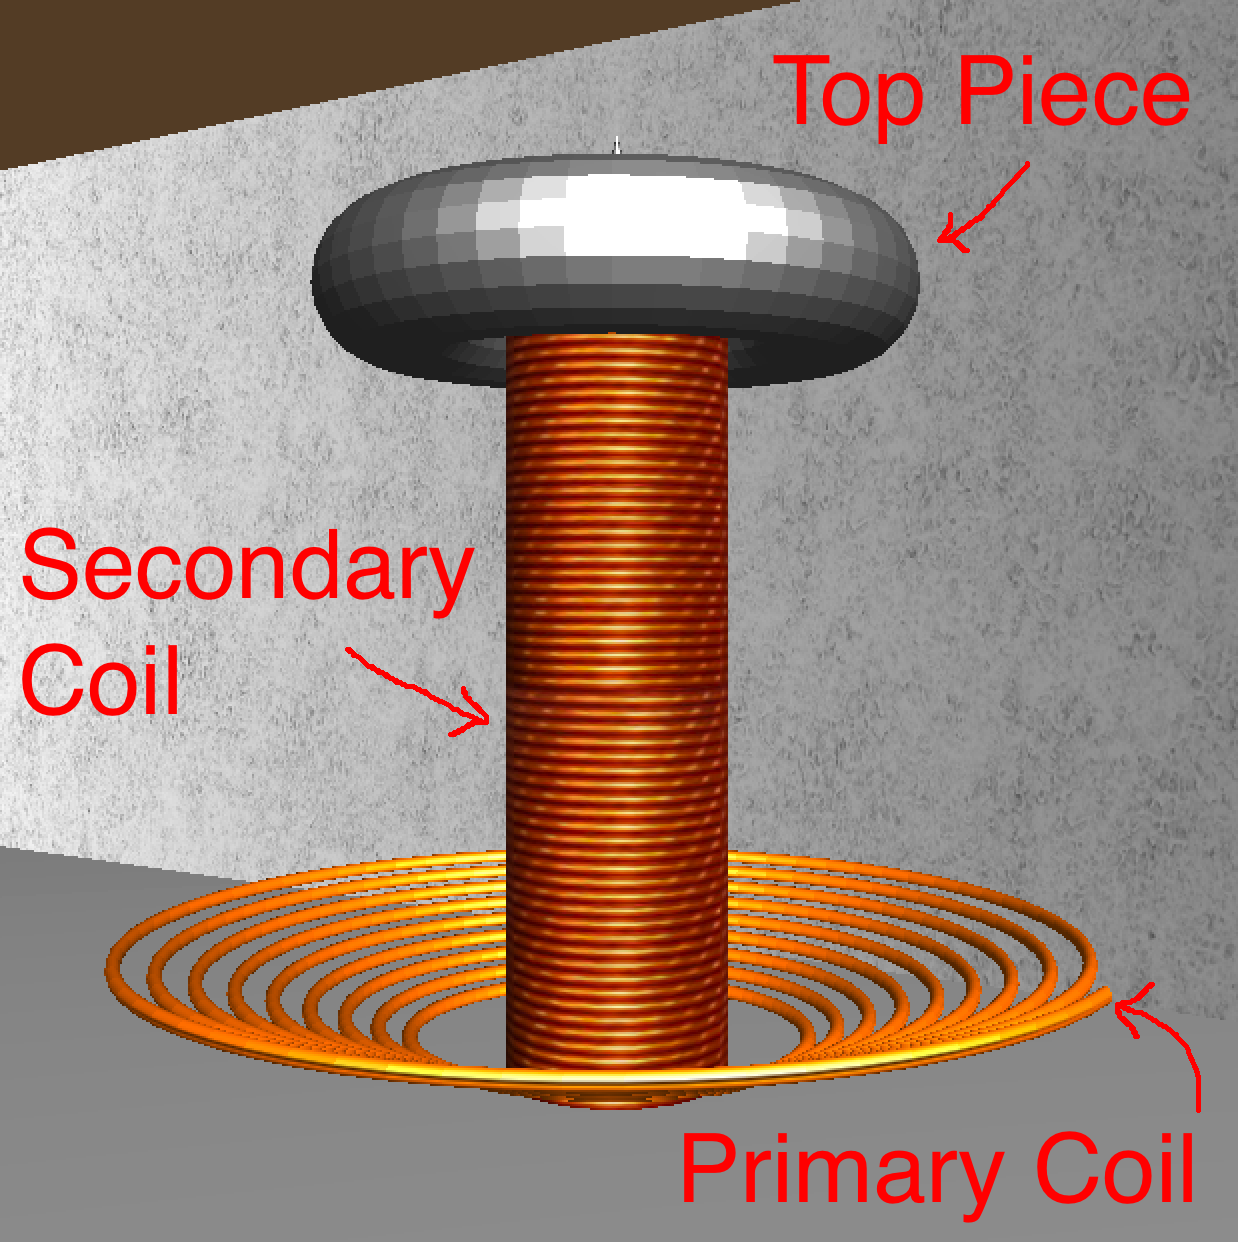
\includegraphics[width=4cm]{coil.png}};
%\end{tikzpicture}

\subsection{Tesla Coil}
The Tesla Coil is constructed in three parts (see figure).  The top piece is an OFF model.  The secondary coil is a textured gluCylinder using mipmaps (since the image has lines).  The primary coil is generated from an equation.  An electricity particle effect is added to the top.
\vspace{2mm}
\newline
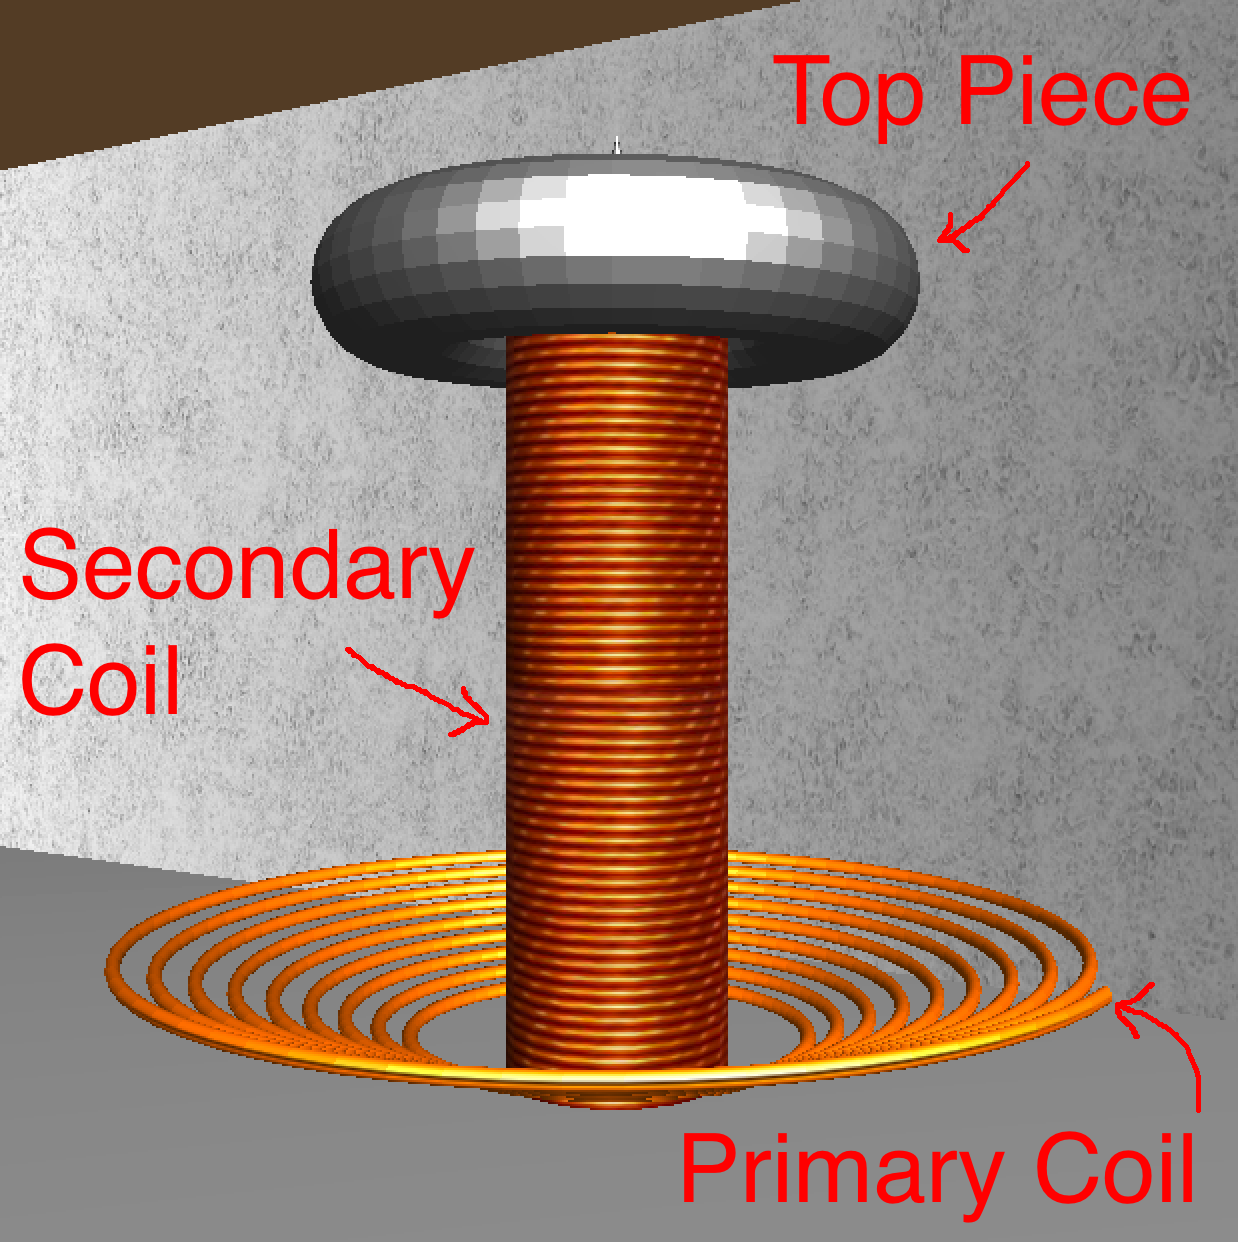
\includegraphics[height=6cm]{coil.png}   % Image
\newline
\newline
\textbf{Feature: Particle System}\hspace{3mm} Each lightning ``bolt'' is drawn on a quad from Targa image file with an alpha channel.  There are 4 distinct lightning bolt graphics.  Instead of having separate files for each, all are taken from a single image file.  A struct holds particle information such as lifespan and how quickly a particle grows or shrinks.  When a particle dies it re-spawns with new randomised values.  There are 4 particles alive at any given time, but this could be increased to any given number.
\newline
\newline
\textbf{Feature: Mathematical Formula}\hspace{3mm} The primary coil spiral is a circle (mathematically generated) quad strip that is swept around the origin at radius $r$ using the polar equation
\begin{equation}
r = a\theta + c
\end{equation}
converted to cartesian coordinates.  And at height
\begin{equation}
y = b\theta
\end{equation}
No glut matrix manipulation functions were used.

\newpage
\subsection{Electromechanical oscillator}
The oscillator exhibit has 3 parts; the white glut primitives, the grey steel bar that moves up and down and the oscillator that is fixed to the centre of the bar.  The bar curves in the centre while both ends of the bar remain rigid.
\vspace{2mm}
\newline
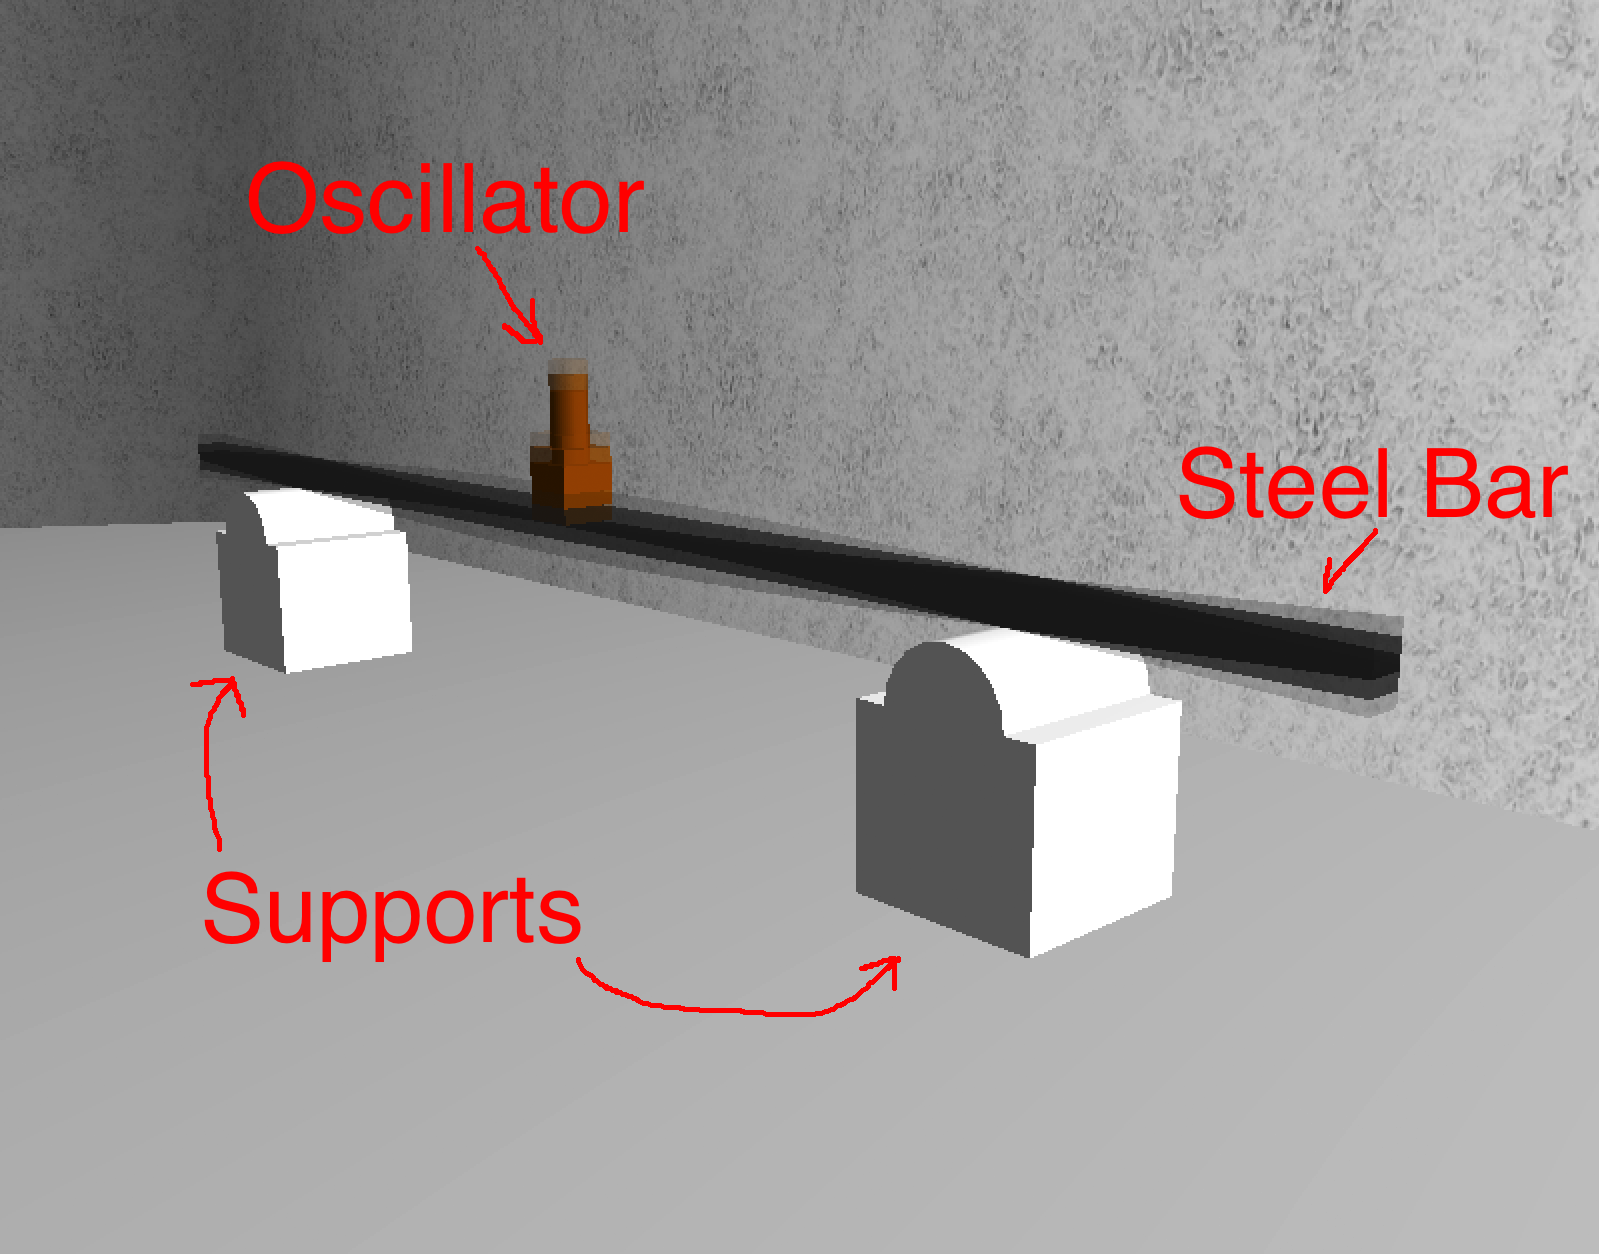
\includegraphics[height=6cm]{oscillator.png}
\newline
\newline
\textbf{Feature: Mathematical Formula}\hspace{3mm} There are 3 equations associated with the bar's movement.  The curvature of the bar is determined by a sine function.  The frequency that the bar moves at is another sine function.  The change in maximum amplitude of the bar's oscillation follows a normal distribution, A.K.A bell curve\textsuperscript{[2]}.
\begin{equation}
f(x) = \frac{1}{\sigma\sqrt{2\pi}} e^{-(x - \mu)^{2}/(2\sigma^{2}) }
\end{equation}

\subsection{Skybox}
The skybox in the scene is 4 textures mapped on the inside of a large cube.  The focal length was chosen to minimise distortion at the edges.

\subsection{Mipmaps}
Mipmaps were implemented by adding a number to the end of filenames corresponding to the mipmap level.  The loadBMP function loads all mipmap textures recursively.  The textures using mipmaps are: the outside of the museum, the portrait of Nikola Tesla and the copper winding texture on the cylinder of the tesla coil.  These textures were distorted at a distance without mipmapping.

\section{References}
1. Eight Curve \textcolor{blue}{\url{https://mathworld.wolfram.com/EightCurve.html}} \newline
2. Normal Distribution \textcolor{blue}{\url{https://mathworld.wolfram.com/NormalDistribution.html}}
\newline
3. Textures from \textcolor{blue}{\url{https://www.textures.com/}}  % (see article 6 \& 7 \textcolor{blue}{\url{https://www.textures.com/terms-of-use.html for licence}})
\newline
4. Coil Texture from \textcolor{blue}{\href{http://polymericinsulators.m.sell.fnxradio.com/pz6904fc0-film-sintering-enamel-coated-copper-wire-for-motor-winding-high-power.html}{link}}
\newline
5. Skybox textures  \textcolor{blue}{\url{https://learnopengl.com/Advanced-OpenGL/Cubemaps}}
\newline
6. Nikola Tesla image Unknown author / Public domain
\newline
7. All other Models and textures created by me













\end{document}  